
\documentclass[twocolumn]{article}
\usepackage{mathpazo}
\usepackage{microtype}
\usepackage{times}

 %%%%%%%%%%%%%%%%%%%%%%%%%%%%%%%%%%%%%%%%%%%%%%%%%%%%%%%%%%%%%%%%%%%%%%%%%%%%%
 %                              My Commands
\newcommand{\bi}{\begin{itemize}}
\newcommand{\ei}{\end{itemize}}
\newcommand{\be}{\begin{enumerate}}
\newcommand{\ee}{\end{enumerate}}
\newcommand{\ii}{\item}
\newtheorem{Def}{Definition}
\newtheorem{Lem}{Lemma}
\usepackage{algorithm}
\usepackage{algorithmicx}
\usepackage{algpseudocode}

\usepackage{graphicx}
\graphicspath{%
        {converted_graphics/}
        {./images/}
}
    
\setlength\textwidth{7in} 
\setlength\textheight{9.5in} 
\setlength\oddsidemargin{-0.25in} 
\setlength\topmargin{-0.25in} 
\setlength\headheight{0in} 
\setlength\headsep{0in} 
\setlength\columnsep{18pt}
\sloppy 
 
\begin{document}

\title{
\vspace{-0.5in}\rule{\textwidth}{2pt}
\begin{tabular}{ll}\begin{minipage}{4.75in}\vspace{6px}
\noindent\large Autonomous Control Middleware Research Section\\
\vspace{-12px}\\
\noindent\LARGE ETRI\qquad \large Technical Report 13VC1310-TR-06
\end{minipage}&\begin{minipage}{2in}\vspace{6px}\small
218 Gajeong-ro, Yuseong-gu\\
Daejeon, 305-700, South Korea\\
http:/$\!$/www.etri.re.kr/\quad 
\end{minipage}\end{tabular}
\rule{\textwidth}{2pt}\vspace{0.25in}
\LARGE \bf
Imaging Earth's Subsurface Using CUDA
}

%\date{Autonomous Control Middleware Research Section, ETRI}

\author{
{\bf Sung-Soo Kim}\\
\it{sungsoo@etri.re.kr}
}

\maketitle

\begin{abstract}
Companies in the oil and gas industry depend on accurate seismic surveys of the Earth to identify subsurface oil reservoirs. The challenge is that most seismic data sets are many terabytes in size and it takes enormous amounts of computing power to convert the raw data into useful survey images.
This technical report describes a CUDA implementation of several time-critical algorithms within industrial seismic processing pipeline. This CUDA implementation achieves significant performance improvements over the latest generation of CPUs, and this reports presents the possibility of building clusters of GPUs to accelerate large seismic processing problems.

\end{abstract}

\section{Introduction}
The main goal of earth exploration is to provide the oil and gas industry with knowledge of the \emph{earth's subsurface structure} to detect where oil can be found and recovered. To do so, large-scale seismic surveys of the earth are performed, and the data recorded undergoes complex iterative processing to ex‐ tract a geological model of the earth. The data is then interpreted by experts to help decide where to build oil recovery infrastructure.

The state-of-the-art algorithms used in seismic data processing are evolving rapidly, and the need for computing power increases dramatically every year. For this reason, CGGVeritas has always pioneered new \emph{high-performance computing} (HPC) technologies, and in this work we explore GPUs and NVIDIA's CUDA programming model to accelerate our industrial applications.

The algorithm we selected to test CUDA technology is one of the most resource-intensive of our seismic processing applications, usually requiring around a week of processing time on a latest-generation CPU cluster with 2,000 nodes. To be economically sound at its full capability for our industry, this algorithm must be an order of magnitude faster. At present, only GPUs can provide such a performance break‐ through.

After much analysis and testing, we were able to develop a fully parallel prototype using GPU hardware to speed up part of our processing pipeline by more than a factor of ten. In this chapter, we present the algorithms and methodology used to implement this seismic imaging application on a GPU using CUDA. It should be noted that this work is not an academic benchmark of the CUDA technology—it is a feasibility study for the industrial use of GPU hardware in clusters.

\section{Geological Background}
An important part of today's search for hydrocarbon reservoirs such as oil and gas is the use of seismic methods which measure changes in acoustic impedance to explore the interior of the earth. The \textit{visualization} and \textit{interpretation} of the resulting information is a challenging task due to the huge amount of generated data, which can easily reach sizes of multiple gigabytes. Moreover, seismic data contains a high presence of noise, which makes it even more difficult to visualize. Interpretation often includes time-consuming manual tasks by so-called \textit{seismic interpreters} to identify subsurface structures that may hint at potential hydrocarbon deposits.

\subsection{Formation of Petroleum Deposits}
Natural oil and gas fields develop over long periods of time, slowly transforming organic matter through chemical conversion processes into hydrocarbons. Dead marine organisms such as algae accumulate over hundreds of thousands of years on the sea floor, building sediment stratas with a high proportion of organic material. Over time more and more sediments are deposited on top of the organic layer, creating higher pressures and temperatures. 
Under these effects of pressure and heat the hydrocarbons that are contained in the biomass distill into crude oil or natural gas. Rocks that contain accumulated amounts of these distilled hydrocarbons are called \textit{source rocks}.

If sediment layers above a source rock are porous and permeable the interstitial oil may flow out of the rock and travel through more porous limestone or sandstone until it reaches a \textit{reservoir} or is blocked by an impermeable layer. This process of movement is called \textit{petroleum migration} and is caused by hydrology, fluid pressures and water movement. 
Once the movement of oil or gas has come to an end because it reached an impermeable sediment layer, it is said to be trapped and the geological structure that causes the end of the hydrocarbon migration is called \textit{petroleum trap}. 
\begin{figure}[htb]
        \centering
        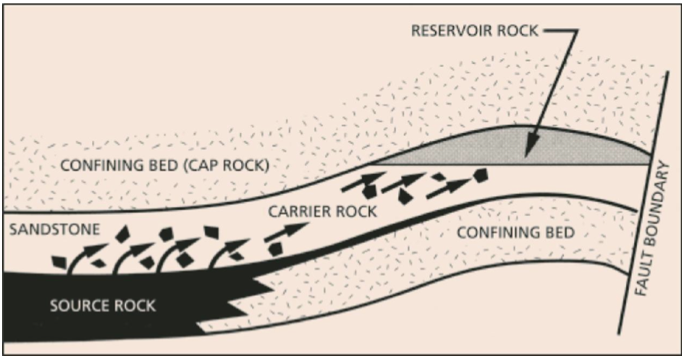
\includegraphics[width=0.48\textwidth]{oilmigration}
        \caption{Oil migration from source into reservoir rock}
        \label{migration}
\end{figure}

There are four main groups of geological structure in which hydrocarbons can be trapped: \textit{anticlines}, \textit{salt domes}, \textit{faults} and \textit{unconformities} (Figure \ref{migration}). However for deposits to develop several conditions must be fulfilled. A source rock must be present and located within a suitable geometrical and historical relations to a reservoir or a trap. Moreover there must be a migration pathway that actually allows the petroleum to travel into the reservoir. The fact that source rock and petroleum trap can be separated by very long distances makes the detection of reservoirs even more complicated. It can be seen that the accurate detection of such geological features is a complicated task since no direct picture of the subsurface can be taken. Information on the inner depths of the earth must be derived from results of different geophysical measurements.

\section{Survey Techniques}
The most unambiguous tool for locating hydrocarbon reservoirs is to drill. However the process of drilling requires an enormous financial investment and is extremely labor intensive. Moreover, drilling blindly into the subsurface carries great risks for nature and possibly also the human population and therefore it is crucial to obtain as much information as possible on the target area to be able to properly prepare a drilling operation. 
\begin{figure}[htb]
        \centering
        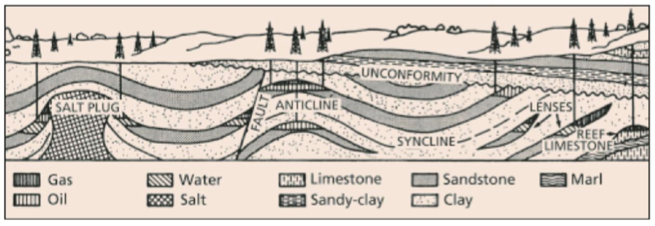
\includegraphics[width=0.48\textwidth]{hydrocarbon}
        \caption{Different types of hydrocarbon traps.}
        \label{hydrocarbon}
\end{figure}

Geophysical surveys cover a wide range of techniques and processes that aim at reducing the potential risks and maximize the profit outlook of drilling operations. Survey techniques can be classified as either \textit{active} or \textit{passive} depending on whether they make use of fields that occur naturally or whether they take measurements of artificially generated energy. Examples of natural fields are the gravitational, magnetic, electrical or electromagnetic fields of the earth.

Artificially generated sources can be the generation of local electrical or electromagnetic fields or most importantly in the context of hydrocarbon exploration seismic waves that are used to explore the inner depths of the earth. Geophysical methods are generally used in a complementary sense, since none of the techniques delivers unambiguous evidence of the subsurface. For example the beginning of a survey might be done by airborne-based gravi- metric and magnetic measurements. Based on the findings of these measurements certain areas can be identified where more detailed seismic surveys are carried out subsequently.

\subsection{Seismic Survey Techniques}
Seismic techniques are the most widely used type of examination method in the area of petroleum exploration. The basic principle of seismic measurements is very similar to the one of \textit{ultrasound imaging}, which produces images of the interior of a human body using very high frequency sonic pulses. 
In contrast to the very short wavelength of ultrasound, seismic methods use far lower frequencies resulting in much longer wavelengths. So one major difference between the two techniques is the \textit{distance}, which the sound waves can travel into the source object. High-frequency ultrasound penetrates a human body in the centimeter range, whereas the low-frequency seismic pulses can reach depths of several thousand meters inside the earth. To perform a seismic measurement it is necessary to generate an artificial low-frequency sound wave at the surface level. This wave will travel down into the earth and will be partially refracted and reflected at the interfaces between different rock layers. Each time a wave hits an interface it is split and partitioned into two reflected and two refracted waves.

In the context of reflection seismology this is called a \textit{seismic event}. The reflected energy travels back to the surface and is registered by multiple arrays of geophones. During this process two important properties can be measured.

\subsection*{Two Way Travel Time}
The first is the amount of time it takes for the wave to travel down to the reflector and back up to the receiver. This temporal information is related to the \textit{depth} of a reflector and is known as \textit{two way travel time} (TWTT). However only reflections that are below 50 feet can be detected clearly because arrival times of reflectors above that depth are nearly the same as the much stronger direct ground reflection. Reflections of deeper interfaces will arrive at the geophones later and after the peak amplitude of the ground reflection has passed, which makes them easier to detect.

\subsection*{Reflection Strength}
The second value is \textit{the strength of the reflected signal}, which is an indicator of the properties of rock change at the reflecting interface. 
The amount of energy that is reflected at an interface depends on the contrast in \textit{impedance} between two overlying layers. 
\textit{Acoustic impedance} is defined as the product of density and seismic velocity in a certain rock layer and is measured in distance per second. Seismic velocity is the propagation velocity of a seismic wave for a given medium and depends on multiple factors such as porosity, lithology, interstitial fluids or depth. For example since rock density tends to increase with depth, the speed of seismic waves also becomes faster the deeper a wave has penetrated into the earth. Table \ref{velocity} contains average wave velocities for materials that are commonly contained in the interior of the earth.
\begin{figure}[htb]
        \centering
        \includegraphics[width=0.48\textwidth]{velocity}
        \caption{Average seismic velocities for common materials}
        \label{velocity}
\end{figure}

Seismic measurements do not directly locate the position of hydrocarbon reservoirs but instead deliver important \textit{structural} information that can be used to infer the presence or absence of oil and gas. This is due to certain properties such as source rock maturity or migration pathways not being detectable in seismic data. Seismic techniques are therefore sometimes described as \textit{indirect exploration techniques}. 
Nevertheless nowadays the seismic method is by far the most widely used technique in the field of geophysical exploration.

\section{Seismic Data}
\subsection{Seismic Waves}
\textit{Reflection seismology} uses artificially generated seismic waves to explore the inner depths of the earth. Since these seismic waves are ordinary sound waves they spread out in all directions when traveling through a medium. The speed of propagation depends on the density of a material. The points of a wave that have traveled for the same amount of time are called \textit{wavefront}. In a uniform medium the wavefront of a seismic wave has a spherical shape with all points of the wave being equidistant from the source (Figure \ref{seismicwaves}). Points on a wavefront share the amount of time they have traveled but not necessarily the same amount of distance, as the propagation speed may vary due to different rock densities within the subsurface. Seismic waves can be divided into two main groups, \textit{body waves} and \textit{surface waves}.
\begin{figure}[htb]
        \centering
        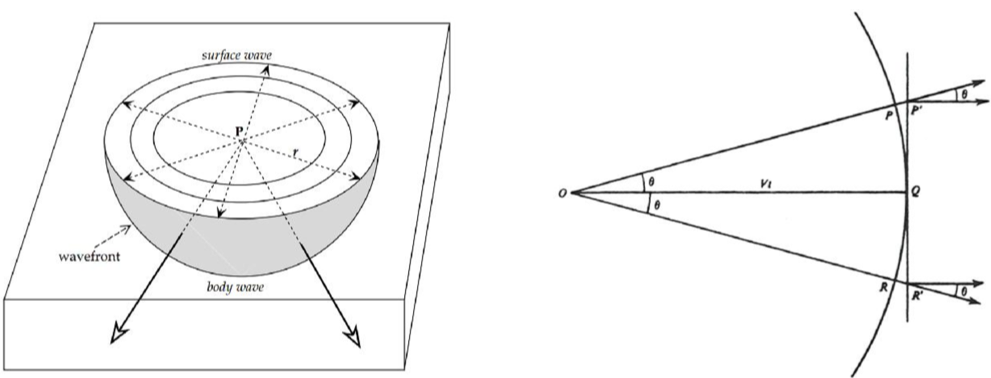
\includegraphics[width=0.48\textwidth]{seismicwaves}
        \caption{Propagation of a seismic wave from a point source P near the surface of a uniform medium (left). A spherical wavefront can be approximated by a planar wavefront (right) }
        \label{seismicwaves}
\end{figure}
\subsubsection*{Body Waves}
Body waves can occur either as \textit{compressional waves} (longitudinal, primary or P-wave) or as \textit{shear waves} (transversal, secondary or S-wave). Compressional waves move through a medium by axial deformation of the medium in the direction of wave propagation. This de- formation consists of consecutive compressions and dilatations of the transmission medium. Shear waves propagate by a shear displacement that is perpendicular to the direction of the wave. Because compressional waves will always travel faster than shear waves in the same medium they arrive at the receiver first and are hence also known as primary waves. Unlike compressional waves that can propagate in any kind of medium (solids, liquids and gases), shear waves can only propagate through solid materials. This characteristic leads to the assumption that the outer core of the earth is liquid since no shear waves can travel through it. Figure \ref{displacement} illustrates the displacement patterns for different types of seismic waves.
\begin{figure}[htb]
        \centering
        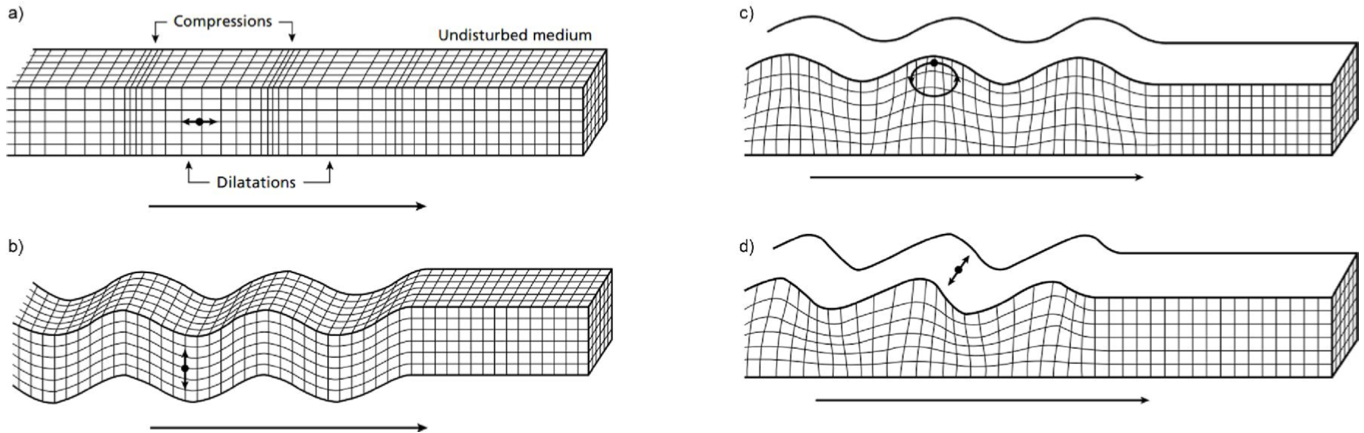
\includegraphics[width=0.48\textwidth]{displacement}
        \caption{Displacement patterns for different wave types. Compressional waves (a), shear waves (b), Rayleigh waves (c) and love waves (d).}
        \label{displacement}
\end{figure}

\subsubsection*{Surface Waves}
In contrast to body waves that spread out into the subject medium, surface waves travel in parallel along the boundary of a solid. 
In a geophysical context this means the crust of the earth. The name comes from the circumstance, that surface waves are tied to the surface and attenuate with distance from the surface. This means that amplitude and particle motion decrease rapidly with increasing depth. However since surface waves only propagate in two dimensions, they lose less energy and therefore decay more slowly compared to body waves, which propagate in three dimensions. There are two types of surface waves that are of importance in the context of \textit{reflection seismology}, \textit{Rayleigh waves} and \textit{Love waves} (Figure \ref{displacement}). The former propagate similar to waves on the surface of an ocean. The transmission medium is moved up and down and side to side perpendicular to the direction of the wave. This includes longitudinal as well as transversal particle motions. The latter are the fastest moving surface waves and propagate by horizontal shifting of the earth and are sometimes described as \textit{polarized shear waves}. Surface waves travel generally with a slower velocity compared to body waves.

\subsubsection*{Seismic Raytracing}
Determining the exact propagation paths (thus the wavefront) of a seismic wave through a \textit{heterogeneous medium} such as subsurface geology is an extremely difficult task. In order to simplify the calculations the following mathematical simplifications are applied. 
One observation that can be made when looking at the spreading of a spherical wave is that the \textit{curvature} of the wavefront decreases with distance from the source. At great distances the radius becomes very large and an infinitesimal small section of the wavefront approaches a \textit{plane wave}. This is illustrated in Figure \ref{seismicwaves}. Since these are simpler to visualize and to express mathematically seismic waves are generally treated as plane waves.

The second simplification is that the direction of wave propagation can be described by \textit{rays} which are perpendicular to the wavefront and point away from the source of the wave. These imaginary rays are called \textit{seismic ray paths} and the process of tracking the propagation of these rays through a given medium is called \textit{seismic ray tracing}. The method of seismic ray tracing is used to generate structural subsurface models based on calculated and observed travel times of both \textit{refracted} and \textit{reflected} seismic disturbances. Since the same concepts that describe reflection and refraction of light rays are also valid for seismic energy, studying the ray paths can deliver evidence on the position or shape of certain subsurface structures.

\subsection{Seismic Volumes}
\subsubsection*{Seismic Traces}
\subsubsection*{Seismic Lines and Volumes}



A \emph{seismic survey} is performed by sending compression waves into the ground and recording the reflected waves to determine the subsurface structure of the earth. In the case of a marine survey, like the one shown in Figure \ref{acquisition}, a ship tows about ten cables equipped with recording systems called \emph{hydrophones} that are positioned 25 meters apart. Also attached to the ship is an air gun used as the source of the compression waves.

\begin{figure}[htb]
        \centering
        \includegraphics[width=0.48\textwidth]{acquisition}
        \caption{Marine Seismic Data Acquisition}
        \label{acquisition}
\end{figure}
A vessel fires an air gun to generate a compression wave that propagates down to the earth and generates reflection waves recorded by hydrophones attached to cables behind the ship.

To acquire seismic data, the ship fires the air gun \emph{every 50 meters}, and the resulting compression waves propagate through the water to the sea floor and beyond into the subsurface of the earth. When a wave encounters a change of velocity or density in the earth media, it splits in two, one part being reflected back to the surface while the other is refracted, propagating further into the earth (see Figure 38-1). Therefore, each layer of the subsurface produces a reflection of the wave that is recorded by the hydrophones. Because sound waves propagate through water at about 2,500 m/s and through the earth at 3,000 to 5,000 m/s, recording reflection waves for about four seconds after the shot provides information on the earth down to a depth of about 10 to 20 km.

A typical \emph{marine survey} covers a few hundred square kilometers, which represents a few million shots and several terabytes of recorded data. Processing this amount of data for many studies in parallel is the core business of CGGVeritas processing centers throughout the world. Due to its very low initial signal- to-noise ratio and the large data size, seismic data processing is extremely demanding in terms of processing power. As illustrated by the image in Figure \ref{capability}, CGGVeritas computing facilities consist of PC clusters of several thousand nodes, providing more than 300 teraflops of computing power and petabytes of disk space.

\begin{figure}[htb]
        \centering
        \includegraphics[width=0.49\textwidth]{capability}
        \caption{Computing Capability Is a Critical Aspect of Our Domain}
        \label{capability}
\end{figure}

To support increasing survey sizes and processing complexity, our computing power needs to grow by more than a factor of two every year (see the graph in Figure \ref{capability}). Furthermore, heat limitations have forced CPU manufacturers to limit future clock frequencies to around 4 GHz. Increasing the size of clusters in data centers can be realistic for only a short period of time, and this problem enforces the need for new technologies. Therefore, we believe mastering new computing technologies such as general- purpose computing on GPUs is critically important for the future of seismic data processing.


\section{Seismic Processing}
The goal of seismic processing is to convert terabytes of survey data into a \emph{3D volume description} of the earth's subsurface structure. A typical data set contains billions of vectors of a few thousand values each, where each vector represents the information recorded by a detector at a specific location and specific wave shot.

The first step in seismic data processing is to \emph{correctly position all survey data} within a global geographic reference frame. In a marine survey, for instance, we need to take into account the \emph{tidal} and \emph{local streams} that shift the acquisition cables from their theoretical straight-line position, and we also need to
include any movement of the ship's position. All of the data vectors must be positioned inside a 100 km2 region at a resolution of 1 meter. Many different positioning systems, both relative and global, are used during data acquisition, and all such position information is included in this processing step.

After correcting the global position for all data elements, the next step is to apply signal processing algorithms to normalize the signal over the entire survey and to increase the \emph{signal-to-noise ratio}. Here we correct for any variation in hydrophone sensitivity that can lead to non-homogeneous response between different parts of the acquisition cables. \emph{Band-limited deconvolution algorithms} are used to verify the known impulse response of the overall acquisition process. Various filtering and artifact removal steps are also performed during this phase. The main goal of this step is to produce data that coherently represents the \emph{physics of the wave reflection} for a standard, constant source.

\subsection{Deconvolution}
n mathematics, deconvolution is an algorithm-based process used to reverse the effects of \textit{convolution} on recorded data.
The concept of deconvolution is widely used in the techniques of \textit{signal processing} and \textit{image processing}. 
Because these techniques are in turn widely used in many scientific and engineering disciplines, deconvolution finds many applications.
In general, the object of deconvolution is to find the solution of a convolution equation of the form:
$$ f * g = h$$
Usually, $h$ is some recorded signal, and $f$ is some signal that we wish to recover, but has been convolved with some other signal g before we recorded it. 
The function $g$ might represent the \textit{transfer function} of an instrument or a driving force that was applied to a physical system. If we know $g$, or at least know the form of $g$, then we can perform deterministic deconvolution. However, if we do not know $g$ in advance, then we need to estimate it. This is most often done using methods of \textit{statistical estimation}.

In physical measurements, the situation is usually closer to
$$(f * g) + \varepsilon = h $$

In this case $\varepsilon$ is \textit{noise} that has entered our recorded signal. If we assume that a noisy signal or image is noiseless when we try to make a statistical estimate of $g$, our estimate will be incorrect. 
In turn, our estimate of $f$ will also be in‐ correct. 
The lower the signal-to-noise ratio, the worse our estimate of the deconvolved signal will be. 
That is the reason why inverse filtering the signal is usually not a good solution. 
However, if we have at least some knowledge of the type of noise in the data (for example, white noise), we may be able to improve the estimate of $f$ through techniques such as Wiener deconvolution.

The foundations for deconvolution and time-series analysis were largely laid by Norbert Wiener of the Massachusetts Institute of Technology in his book \textbf{\textit{Extrapolation, Interpolation, and Smoothing of Stationary Time Series}} (1949).
The book was based on work Wiener had done during World War II but that had been classified at the time. 
Some of the early attempts to apply these theories were in the fields of weather forecasting and economics.



The last and the most important and time-consuming step is designed to correct for the effects of \textit{changing subsurface media velocity }on the wave propagation through the earth. Unlike other echoing systems such as radar, our system has no information about the propagation velocity of the media through which the \emph{compression waves} travel. Moreover, the media are not homogeneous, causing the waves to travel in curves rather than straight lines, as shown in Figure 38-3a. Therefore, the rather simple task for radar of converting the time of the echo arrival into the distance of the reflection is, in the seismic domain, an extremely complex, inverse problem. To further complicate the process, more than one reflection occurs after a wave shot, so the recorded signal can in fact be a \emph{superposition} of many different reflections coming from different places.

\begin{figure}[htb]
        \centering
        \includegraphics[width=0.49\textwidth]{reflector}
        \caption{Ray Tracing for a Single Reflector Through the Earth, Modeled by a Velocity Field Display in Color \small{\emph{(a) We can clearly see how velocity variations bend the rays even for a rather smooth velocity model. (b) In some cases, the velocity changes are extremely complex and nonhomogeneous, and the wave propagation is extremely difficult to model, escpecially because we would need to compute billions of rays.}}}
        \label{reflector}
\end{figure}

Because the velocity field is initially unknown, we generally start by assuming a rather simple velocity model. Then the \textit{migration process} gives us a better image of the earth's subsurface that allows us to re‐ fine the velocity field. This iterative process finally converges toward our best approximation to the ex‐ act earth reflectivity model.

At the end of the processing, the 3D volume of data is far cleaner and easier to understand. Some attributes can be extracted to help geologists interpret the results. Typically the impedance of the media is one of those attributes, as well as the wave velocity, the density, and the anisotropy. Figure \ref{seismic} gives an overview of what the data looks like before and after the processing sequence. Also shown is an \textit{attribute map} representing the wave velocity at a particular depth of the seismic survey. Different rock types have different velocities, so \textit{velocity is a good indicator} to look for specific rocks such as sand. In the particular case of Figure \ref{seismic}c, \textit{low velocities }(in blue) are characteristic of \textit{sand}, here from an old riverbed. As a rock, sand is very porous and is typically a good location to prospect for oil.

\begin{figure}[htb]
        \centering
        \includegraphics[width=0.49\textwidth]{seismic}
        \caption{A Seismic Processing Example \small{\emph{ (a) Raw data recorded during a land survey in Germany showing the poor signal-to-noise ratio and the lack of calibration. (b) A vertical section of about 10 km wide and 5 km deep in the final 3D result shows the layered structure of the earth. (c) This map represents an attribute extracted at a particular depth from a final seismic data set. This attribute is used to distinguish between sand and shale rocks (blue versus green) around a winding shape, which is the remaining channel imprint of a 70-million-year-old river buried under 10 km of earth.
	}}
	}
        \label{seismic}
\end{figure}

\subsection{Wave Propagation}
For a perfect theoretical seismic data set, the recorded signal $r_x$ of the wave propagation from a specific source $S_i$ recorded by a hydrophone $G_j$ after a reflection of amplitude $R_x$ at the 3D location$ x(x, y, z)$ can be expressed as follows:
\begin{equation}
r_x = P^V_{xy}(R_x \cdot P^V_{ix}(W_s)),
\label{equ01}
\end{equation}

where $W_s$ is the source signal, $P_{ix}$ is the operator that propagates the wave from the source position $i$ to the reflection position $x$ through the velocity field $V$, and $P_{xj}$ is the operator that propagates the reflected wave from $x$ to the recorder position $j$.
To model the complete seismic recording by one receiver, we need to integrate the Equation \ref{equ01} for all possible reflection positions—that is, integrate on the whole 3D volume of x values:
\begin{equation}
S_j = \int_x [P^V_{xj}(RC_{earth}(x) \cdot P^V_{ix}(W_x))],
\label{equ02}
\end{equation}

where $S_j$ is the seismic recording at position$j$ and $RC_{earth}$ is the reflectivity model of the earth we are looking for. The complexity should be apparent now, because each of the hundreds of millions of data vectors may include information from the whole earth area in a way that depends on the velocity field. Note that in practice the velocity is around a few kilometers per second. Thus if we record wave reflection for a few seconds, only the earth approximately 10 km around the receiver position will contribute to the signal.

It is not realistic to use a brute-force approach to solve this inverse problem, but it can be simplified if we use the property of the propagation operator: $P_{ij} (Pji (a)) = I$. That is, propagation from source to reflection point and back to the source position should give the initial result (that is, there should be no dissipation). From Equation \ref{equ01} we can see that

\begin{equation}
P^V_{jx}(r_x) = P^V_{jx}(P^V_{xy}(R_x \cdot P^V_{ix} (W_s))) = R_x \cdot P^V_{ix}(W_s).
\label{equ03}
\end{equation}

And if we consider all the possible contributions to a specific record--that is, summing up all contributions for all $x$ locations--we can write this:
\begin{equation}
\int_x P^V_{jx}(S_j) = \int_x[RC_{earth}(x) \cdot P^V_{ix}(W_s)]  = RC_{earth} \otimes \int_x[P^V_{ix}(W_s)].
\label{equ04}
\end{equation}

Hence, the recorded seismic signal $S_j$ , taken as a source and propagated through the earth at all possible x locations, is equal to the earth reflectivity model convolved by the initial source shot propagated to any possible reflection position in the earth. It is then clear that if we correlate both sides of this equation by $\int_x[P^V_{ix}(W_s)]$ and sum up information from all receivers for each source, we may extract the earth reflectivity model:
$$RC_{earth} = \sum_s[\int_x P^V_{ix}(W_x)*\sum_j \int_x P^V_{jx}(S_j)],$$
where * is the correlation operator, and using $\int_x[P^V_{ix}(W_s)]*\int_x[P^V_{ix}(W_s)]=1$.

Hence, if we propagate the source wave through the earth to all reachable positions $x$, and correlate
the result with the recorded data back-propagated to the same $x$ location, we only have to sum up results for all sources and all receivers to obtain the earth reflectivity model. Note that in practice we need to take into account the dispersive effect of the propagation, as well as the fact that the data is band limited. Also, because the velocity field is initially unknown, we need to start with an initial guess (based on expert knowledge of the area) to compute a first reflection model and then refine our velocity field by interpreting the results in terms of the geological structure. (See Yilmaz 2001 and Sherifs 1984 for more information.)




























\end{document}
